A relation is a set of inputs and their associated outputs.
To each input there is a corresponding output.
Usually (but not always) we use $x$ for the inputs
and $y$ for the outputs.
In this case, we say that a relation is 
a set of $x$'s and their corresponding $y$'s.

There are several ways to specify a relation:
\begin{itemize}
    \item {\bfseries\itshape ordered pairs}: 
    a set that lists the inputs and corresponding outputs as ordered pairs
    \item {\bfseries\itshape tables}: 
    a table of all the inputs and corresponding outputs
    \item {\bfseries\itshape mappings}: 
    diagrams that use arrows to connect inputs to their corresponding outputs
    \item {\bfseries\itshape graphs}: 
    graphs that plot all the ordered pairs in a 2-D grid 
    (either as a collection of points or, more often, as a curve of infinitely many points)
\end{itemize}


\begin{myExample}{
    Represent the relation
    \(
        \{ (1,2), (3,2), (5,-2), (1,-3) \}
    \)
    as a {\bfseries table}, {\bfseries mapping}, and {\bfseries graph}.
}
    As an input-output table:

    \begin{center}
    \begin{tabular}{cc}
        \toprule
        \emph{inputs} & \emph{outputs} \\
        \midrule
        1 & 2\\
        3 & 2\\
        5 & -2\\
        1 & -3\\
        \bottomrule
    \end{tabular}
    \end{center}

    As a mapping from inputs to outputs:

    \begin{center}
        \(
            1 \longrightarrow 2
        \)\\
        \(
            3 \longrightarrow 2
        \)\\
        \(
            5 \longrightarrow -2
        \)\\
        \(
            1 \longrightarrow -3
        \)
    \end{center}

    As a graph:

    \begin{center}
        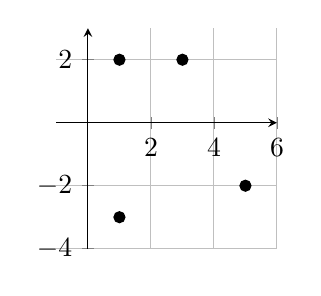
\begin{tikzpicture}
            \begin{axis}[
                width=2in,
                grid=both,
                axis x line = middle,axis y line = middle,
                axis equal image,
                % minor tick num=1,
                xtick distance = 2, ytick distance = 2,
                xmin = -1, xmax=6,
                ymin = -4, ymax=3,
                ]
                \addplot[
                    only marks,
                    mark=*,
                    % mark size = 0.15cm,
                    ] coordinates { (1,2) (3,2) (5,-2) (1,-3) };
            \end{axis}
        \end{tikzpicture}
    \end{center}
\end{myExample}


The \emph{domain} of a relation is the set of all the inputs.
It's all the inputs of the ordered pairs.
Or it's all the inputs in the table or the mapping.
Or it's all the inputs coordinates in the graph.
Since we usually use the variable $x$ for inputs,

\begin{center}
\begin{tcolorbox}[width=3in]
    The {\bfseries\itshape domain} is the set of all the $x$'s.
\end{tcolorbox}
\end{center}

The \emph{range} of a relation is the set of all the outputs.
It's all the outputs of the ordered pairs.
Or it's all the outputs in the table or the mapping.
Or it's all the outputs coordinates in the graph.
Since we usually use the variable $y$ for outputs,

\begin{center}
\begin{tcolorbox}[width=3in]
    The {\bfseries\itshape range} is the set of all the $y$'s.
\end{tcolorbox}
\end{center}


\begin{myConceptSteps}{To find the domain and range of a relation\dots}
    \myStep{inputs}{Write down all the inputs ($x$ values).}
    \myStep{domain}{The domain is those values \emph{without any duplicated values}.}
    \myStep{outputs}{Write down all the outputs ($y$ values).}
    \myStep{range}{The range is those values \emph{without any duplicated values}.}
\end{myConceptSteps}

\begin{myExample}{
    Find the domain and range of this relation:
    \(
        \{ (1,2), (5,6), (3,4) \}
    \)
}
    \vspace{1in}
\end{myExample}

\begin{myExample}{
    Find the domain and range of this relation:
    \begin{center}
        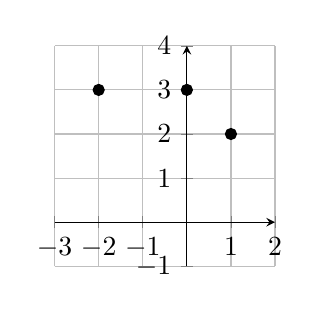
\begin{tikzpicture}
            \begin{axis}[
                width=2in,
                grid=both,
                axis x line = middle,axis y line = middle,
                axis equal image,
                xtick distance = 1, ytick distance = 1,
                xmin = -3, xmax=2,
                ymin = -1, ymax=4,
                ]
                \addplot[
                    only marks,
                    mark=*,
                    % mark size = 0.15cm,
                    ] coordinates { (1,2) (-2,3) (0,3) };
            \end{axis}
        \end{tikzpicture}
    \end{center}
}
    \vspace{1in}
\end{myExample}


